\documentclass[12pt]{article}

%AMS-TeX packages
\usepackage{amssymb,amsmath,amsthm} 
%geometry (sets margin) and other useful packages
\usepackage[margin=1.25in]{geometry}
\usepackage{graphicx,ctable,booktabs}
\graphicspath{ {images/} }


%
%
\newcommand{\course}[2]{\def\courseName{#1} \def\sectName{#2}}
\newcommand{\assn}[1]{\def\assnName{#1}}
\newcommand{\sect}[1]{\def\sectName{#1}}

%
%Fancy-header package to modify header/page numbering 
%
\usepackage{fancyhdr}
\pagestyle{fancy}
%\addtolength{\headwidth}{\marginparsep} %these change header-rule width
%\addtolength{\headwidth}{\marginparwidth}
\lhead{Ying-Yu, Jianchi, Kexin}
%\chead{Problem \thesection} 
\chead{}
\rhead{\thepage} 
\lfoot{\small\scshape \courseName} 
\cfoot{} 
\rfoot{\footnotesize \assnName} 
\renewcommand{\headrulewidth}{.3pt} 
\renewcommand{\footrulewidth}{.3pt}
\setlength\voffset{-0.25in}
\setlength\textheight{648pt}

%%%%%%%%%%%%%%%%%%%%%%%%%%%%%%%%%%%%%%%%%%%%%%%

\begin{document}

\course{Pandemaniac}{}
\assn{Project Report}
\date{\today}
\title{\courseName \sectName \\ \assnName}
\author{Ying-Yu Ho, Jianchi Chen, Kexin Rong}
\maketitle

\thispagestyle{empty}
\section{Division of Work}
\begin{itemize}
\item Ying-Yu Ho: Randomized high-degree design/implementation; Python code optimization; report write-up.
\item Jianchi Chen: Multiplayer Strategy research; Tournament strategy design/implementation; Network characteristics research; report write-up.
\item Kexin Rong: Basic Strategy design/implementation; Distance centrality research; report write-up.
\end{itemize}

\section{Strategy}
\subsection{Basic Strategy: Randomized high degree nodes}
Say there are $p$ players in the game and we want $s$ seeds. Our basic strategy is to calculate the degree of each node in the graph, and randomly choose $s$  from the top $s \times p$ nodes with the largest degrees. \\\\
The rationales are the following: 
\begin{enumerate}
\item We chose ``degree'' as a measure of a node's importance because it is intuitive that nodes with larger degrees are more important in the spread of epidemics. Once we colored a high degree node, the cluster centered around the node is more likely to be colored.
\item We incorporated randomization to avoid colliding with similar strategies from other teams. 
\end{enumerate}

\subsection{Massively-Multiplayer (8+) Strategy: Failed attempt to find clusters}
After participating in several practice rounds, we observed the distinction in results from 2/4-player games and from 8-player games (See Section $<$Observations$>$ for details). Therefore, we came up with the following strategy:
\begin{enumerate}
\item Randomly choose ($s/5$) nodes from the top $s \times p$ nodes with high degrees. Denote them by ``cluster\_heads''. 
\item For each ``cluster\_head'', get 4 of its highest-degree neighbors that are not  cluster\_heads, and put them into seeds list. 
\end{enumerate}
The rationale for this strategy is to increase our chance of coloring ``incascadable clusters''. But the results were not as good  as we had expected. There are two main reasons for that:
\begin{enumerate}
\item Highest-degree neighbours of high-degree nodes tend to be global high-degree nodes themselves, which caused a lot of collision with other players.
\item There aren't many ``real'' clusters, and this simple model can't always find clusters either. 
\end{enumerate}
We gave up the attempt of taking advantage of clusters because it is very hard to implement an efficient algorithm without knowledge of the graph structure to find big clusters.  

\subsection{Another perspective: Distance Centrality}
During the hunt for effective algorithm, we also tried to use the node's average distance to all other nodes as a centrality measure locally. The distances between any two nodes in the graph are computed by Floyd Warshall algorithm. If a node is not connected to all other nodes in the graph, we discard it since this node is more likely to be unimportant.
Since Floyd Warshall algorithm takes $O(n^3)$, we were only planning to use it for graph with fewer nodes. We run this algorithm locally against the randomized-high degree algorithm in simulation, on graphs of 100 nodes and 500 nodes. In each run, the latter won by a large margin (taking over more than 80\% of the nodes). We later found out two main reasons for this result:
\begin{enumerate}
\item Nodes with low average distances (high distance centrality) is also very likely to be of high degrees. Thus, collisions happen inevitably. 
\item For those nodes that have low average distances but not with high-degrees, they ``expand'' themselves much slower than those with high degrees. This will be elaborated in the ``observations'' part. 
\end{enumerate}
Also, since the average distance computation is very time-costly compared to degree measure computation, it is pretty risky to use it for 5000/10000 node graphs. Also, it is hard to add in randomization, since if the random result is not ideal, there is likely no time for a second run. 

\subsection{Beating the TAs: A little cheat on randomized-high-degrees}
One of the tasks in the assignment is to beat the TA strategy. It is observed that the TA strategy is to simply choose the $s$ nodes of highest degrees. Therefore, to beat the TA, we employed the following scheme:
\begin{enumerate}
\item Assuming there are $s$ seeds to be chosen. In each run, we randomly choose $s$ seeds among the $(s+2)$ nodes of highest degrees. 
\item Since we know exactly what the TA-strategy will pick, we also generate a ``rival seed set'' and run the simulation locally against it. 
\item If the randomly chosen set wins, submit the set; otherwise go back to step $1$ and rerun the program. 
\end{enumerate}
This turns out to be simple and effective. A winning set is usually generated after a few runs. 

\subsection{Tournament Strategy: Eggs in different baskets}
As we have decided to base our final strategy on degree centrality, we are also aware that many other teams would do the same, causing inevitable collisions, leaving the result to pure luck. Therefore, we decided that we will use a modified version of randomized-high-degree strategy, described below:
\begin{enumerate}
\item Define the number of players as $p$. Define ``competition factor'' $c \propto p^{-1}$. Define ``stepwidth'' $w \propto p$. Define ``number of steps'' $n$ to be 5. 
\item Starting from a list of nodes sorted by degrees from high to low, we skipped the top $p \times s / c$ nodes because it is highly likely that these nodes will be all chosen by other players, and there is no point in picking them as seeds. Then, starting from the remaining top nodes, randomly pick $s / n$ nodes from the following $s \times w$ top nodes, and then go to the next $s \times w$ nodes in the list, until the seeds list is filled.
\item The chosen result is then locally run against $(p - 1)$ players that uses randomized-high-degree algorithm in the simulator, and we submit the results when a satisfying result is shown (usually in 2 or 3 runs). 
\end{enumerate}
This strategy is based on the observation that in a multiplayer game, a lot of high degree seeds will be chosen by other players. This strategy, while preserving the possibility of acquiring nodes of highest degrees, ensures that we won't be left with 0 node or only very few nodes at start. The strategy is mainly designed to conquer randomized-high-degree algorithm, and is very effective. In almost all tournament graphs we ran locally, the strategy was able to capture over 90\% of the nodes.

\section{Observations on Graph Structure}
Multiple observations are made by looking at the graphs and practice rounds results.
\subsection{Large number of Low degree nodes}
We wrote an analyzer on the practice round graphs, and found two interesting facts:
\begin{enumerate}
\item Roughly 33\% to 50\% of all nodes in the graphs have a degree $\leq 2$. 
\item Among those nodes, roughly 40\% to 50\% have a distance $\leq 2$ to nodes in the top-degree list (the top $s \times p$ nodes). 
\end{enumerate}
What this actually means is that if a player takes over several high-degree nodes, he would quickly take over a large number of low-degree nodes, which is very hard to be conquered once colored, because the current color of the node has 1.5 votes. Therefore, the advantage of using degree centrality over other centralities (degree, betweenness, etc.) is that nodes with high degree will have a quick and direct influence over a large number of low-degree nodes. 
\subsection{Network parameters}
We wrote a simple graph parameter analysis program to analyze several randomly chosen practice graphs, and the results are shown in the following table:
\begin{table}[ht]
\caption{Graph Parameter Analysis Results}
\centering
\begin{tabular}{l c c c c}
\hline\hline
Graph & Avg\ Clustering& Overall\ Clustering & Diameter & Avg\ Diameter \\ 
            & Coefficient         & Coefficient               &  &  \\ 
\hline\hline
8.10.5 & 0.5083 & 0.2773 & 6 & 2.8153\\
4.5.3 & 0.4852 & 0.3655 & 7 & 2.8251\\
4.10.3 & 0.4969 & 0.2899 & 6 & 2.7221\\
2.10.32 & 0.5070 & 0.3563 & 6 & 2.8309\\
2.10.22 & 0.4694 & 0.2899 & 7 & 2.5807\\
\hline
\end{tabular}
\end{table}\\
It can be seen from the above table that all graphs seemed to be generated in the same pattern, and holds similar characteristics:
\begin{enumerate}
\item (Relatively) low clustering coefficients. Recall from HW2 that the social network and coauthorship network graphs have ACC of $>$ 0.74 and OCC of $>$0.43, and the graphs here have much lower clustering coefficient. 
\item Small diameter and small average diameter. The graphs have relatively the same diameter parameters as the social network graphs from facebook.
\end{enumerate}
Because of characteristic 1, it would be ineffective to use betweenness centrality as the basis of our choosing of seeds, since the graphs are relatively less clustered. The attempt to find clusters would also be unsuccessful because of this. 
Because of characteristic 2, using closeness (distance) centrality will also be unwise because the maximum diameter is already pretty low, and the small difference in average distance won't be too relevant. 
The degree centralities, on the other hand, spans a lot wider than the other centralities, as can be seen from the degree-distribution ccdf of 8.10.5 below.
\begin{center}
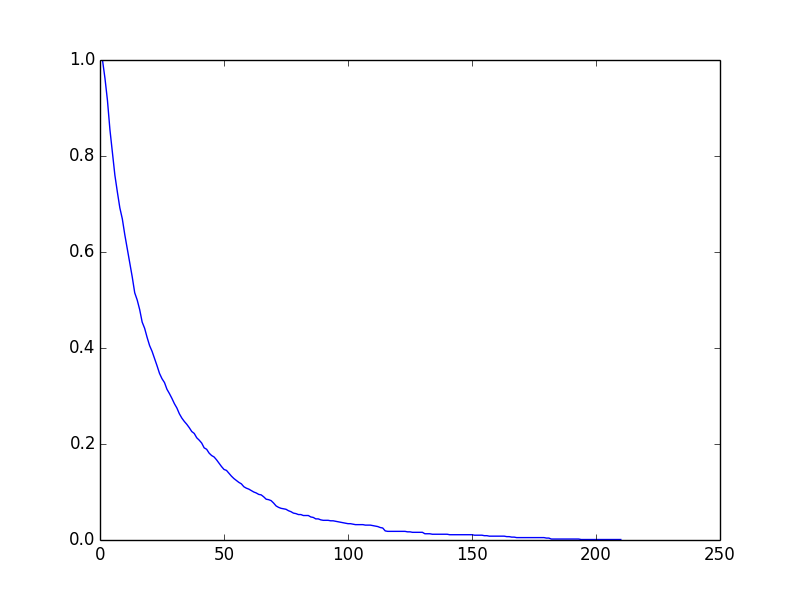
\includegraphics[scale = 0.8]{webgraph_ccdf}
\end{center}
Therefore, it is reasonable to base our strategy on degree centrality measure, instead of other centralities. 


\section{Tournament Results}
In the tournament, we made it through the first round with second highest total score. But we failed in the second round, getting only a total of 13 points in 3 games. This result conveys two messages:
\begin{enumerate}
\item As we have expected, there are at least several teams that employed strategies that involve choosing high-degree nodes, and our strategy was very effective against them. 
\item However, we failed to consider that the teams that made it to the second round are not likely to implement naive strategies, and apparently our strategy was not effective enough against the ``selected'' ones. As can be observed from the resulting graphs, our seeds collide a lot with other teams'.
\end{enumerate}

\section{Counterexample}
The following figure describes a cycle with length 2.\\

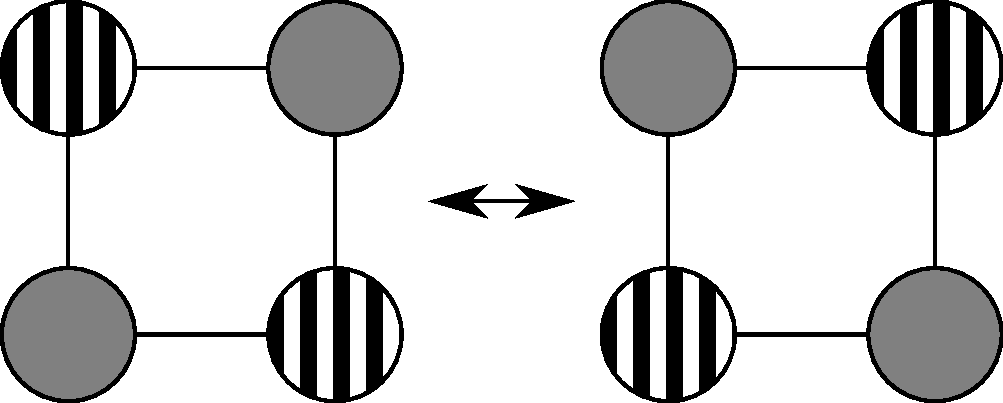
\includegraphics[width=8cm]{counter.pdf}

\section{Suggestions}
\begin{enumerate}
\item Make TA solutions more challenging: \\\\We felt like it didn't take us much work to beat the TAs.  We greatly appreciate the idea that the instructor doesn't want to give the students a hard time. However, making the TAs a little harder to beat can encourage the students to think about more advanced strategies early on, and increase the average "intelligence" of strategies in the whole class.   
\item Increase the variety of graphs: \\\\As we discussed in the observation section, the practice graphs have very similar parameters. We thought that it might be more interesting if the variety of the graphs increases, so that the students need to do more research on the structure of the graphs and can experiment other centrality measures. 
\end{enumerate}


\section{References}
\begin{enumerate}
\item Information Cascade:\\
 http://en.wikipedia.org/wiki/information\_cascade
\item Information Diffusion in Social Media: \\
 http://snap.stanford.edu/class/cs224w-2011/proj/mrom\_Finalwriteup\_v1.pdf

\end{enumerate}


\end{document}